\section{Optimal Transport}%
\label{sec:optimal-transport}
\vspace{1cm}
\begin{figure}[h]%
	\label{fig:paradise}
	\centering
	\fcolorbox{black}{white} {
		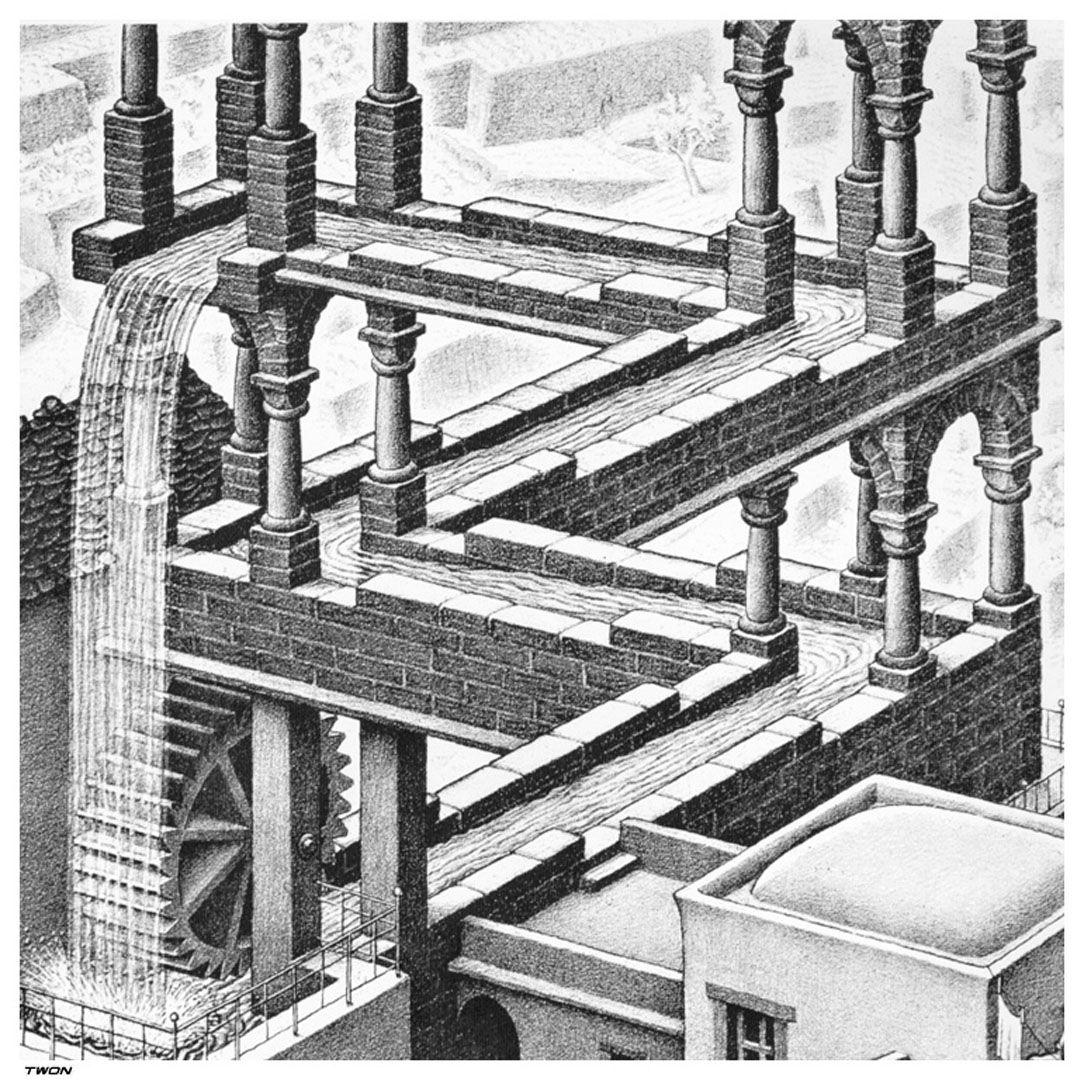
\includegraphics[width=0.3\textwidth]{escher}
	}
	\caption{M.C. Escher's ``Waterfall'' (1961) illustrates an impossible object, symbolizing the challenges in measuring distances between probability distributions.}
\end{figure}
\vspace{1cm}
\noindent In Section~\ref{sec:information-theory}, we explored how the generator minimizes an approximation of the Jensen-Shannon divergence between the true data distribution $p_r$ and the generator distribution $p_g$, which the discriminator approximates at each training step. In this section, we examine the limitations of the value function $\V$ as a GAN objective, stemming from the metric topology induced by the Jensen-Shannon divergence. To address these limitations, we introduce relevant concepts from topology and optimal transport theory, including the earth mover's distance (Wasserstein distance), which forms the foundation of the Wasserstein GAN (WGAN) introduced by~\cite{ref:arjovsky-2017}.

The central insight of this section is that the choice of distance function on a space $\mathcal{X}$ profoundly impacts continuity properties and consequently the ability of sequences of probability distributions to converge within $\mathcal{X}$.

A topological space represents the most general mathematical framework that allows defining continuity and convergence. More specialized spaces like manifolds and metric spaces incorporate additional structure or constraints. A space $\mathcal{X}$ can be equipped with various distance functions, where the open balls form a basis for a topology on $\mathcal{X}$, transforming it into a topological space.

\begin{definition}%
	\label{def:topology1}
	Let $\mathcal{X}$ be any set. A \textnormal{\sffamily topology} $\mathcal{T}$ on $\mathcal{X}$ is a
	collection of subsets of $\mathcal{X}$, each called an open set, satisfying:
	\begin{enumerate}[(i)]
		\item The empty set and $\mathcal{X}$ itself are open;
		\item The intersection of finitely many open sets is open;
		\item The union of any collection of open sets is open.
	\end{enumerate}
	The pair $(\mathcal{X}, \mathcal{T})$ is called a \textnormal{\sffamily topological space}.
\end{definition}

The concept of an open ball is fundamental to the topology of metric spaces. Many useful topological definitions can be formulated using this notion.

\begin{definition}%
	\label{def:open-ball}
	Let $(\mathcal{X}, d)$ be a metric space. An \textnormal{\sffamily open ball} of
	radius $r \in \mathbb{R}^+$ centered at $x_0 \in \mathcal{X}$ is the set
	\begin{align}
		B_d(x_0, r) = \{ x \in \mathcal{X} : d(x, x_0) < r \}.
	\end{align}
	This set contains all points in $\mathcal{X}$ within distance $r$ of $x_0$.
\end{definition}

\begin{definition}%
	\label{def:topology2}
	Let $(\mathcal{X}, d)$ be a metric space. The topology generated by the basis of open
	balls $\mathcal{B} = \{B_d(x, r) \mid x \in \mathcal{X}, r > 0\}$ is called the
	\textnormal{\sffamily topology induced by} $d$ and is referred to as a
	\textnormal{\sffamily metric topology}.
\end{definition}

Different metrics induce different topologies, characterized by their granularity or fineness.

\begin{theorem}%
	\label{thm:granularity}
	Let $d$ and $d^\prime$ be metrics on a set $\mathcal{X}$, and let $\mathcal{T}$ and
	$\mathcal{T}^\prime$ be their respective induced topologies. $\mathcal{T}^\prime$ is
	\textnormal{\sffamily finer} than $\mathcal{T}$ if and only if for each $x \in \mathcal{X}$
	and $\epsilon > 0$, there exists a $\delta > 0$ such that $B_{d^\prime}(x,
		\delta) \subset B_d(x, \epsilon)$.
\end{theorem}

\begin{definition}%
	\label{def:convergence-metric-space}
	Let $\mathcal{X}$ be a finite set of elementary outcomes and $\mathcal{P}$ the space of
	all probability distributions over $\mathcal{X}$ with equal support. Let $d: \mathcal{P}
		\times \mathcal{P} \mapsto \mathbb{R}$ be a metric on this space. A sequence of
	probability distributions $\{(P_n)\}_{n \in \mathbb{N}}$ \textnormal{\sffamily
		converges} to a probability distribution $P$ if $d(P_n,P) \to 0$ as $n \to
		\infty$.
\end{definition}

The Kullback-Leibler and Jensen-Shannon divergences induce a coarser topology than that induced by the earth mover's distance. (See~\cite{ref:arjovsky-2017} for a proof of this statement.) To facilitate convergence, we need a finer topology on $\mathcal{P} \times \mathcal{P}$. A finer topology allows more open sets over $\mathcal{P} \times \mathcal{P}$, making it easier to define continuous maps from $\mathcal{P} \times \mathcal{P}$ to $\mathbb{R}^+$. If a metric $d$ induces a finer topology than another metric $d^\prime$, we say $d$ is a weaker notion of distance than $d^\prime$.

Continuity and convergence can be understood from both topological and metric space perspectives. Below are the relevant definitions from both viewpoints.

\begin{definition}%
	\label{def:continuity-metric-space}
	A function $f: \mathbb{R} \mapsto \mathbb{R}$ is \textnormal{\sffamily continuous} if for
	every $x_0 \in \mathbb{R}$ and $\epsilon > 0$, there exists $\delta > 0$ such that if $|x
		- x_0| < \delta$, then $|f(x) - f(x_0)| < \epsilon$.
\end{definition}

Continuous functions between topological spaces preserve proximity—mapping nearby points in one space to nearby points in the other space.

\begin{definition}%
	\label{def:convergence-topological-space}
	In a topological space $(\mathcal{X}, \mathcal{T})$, a sequence of points
	\textnormal{\sffamily converges} to $x \in \mathcal{X}$ if for every neighborhood $U$
	of $x$, there exists $N \in \mathbb{N}$ such that $x_n \in U$ for all $n \geq
		N$.
\end{definition}

The following is the topological definition of continuity: a function is continuous if the preimage of every open set is open.

\begin{definition}%
	\label{def:pre-image}
	Given a function $f: \mathcal{X} \mapsto \mathcal{Y}$ and a point $y \in \mathcal{Y}$, the
	\textnormal{\sffamily preimage} of $y$ is $f^{-1}(y) = \{x
		\in \mathcal{X} \mid f(x) = y\}$. For any set $A \subset \mathcal{Y}$, the preimage of $A$ is
	$f^{-1}(A) = \{x \in \mathcal{X} \mid f(x) \in A\}$.
\end{definition}

\begin{definition}%
	\label{def:continuity-topological-space}
	Let $\mathcal{X}$ and $\mathcal{X}^\prime$ be topological spaces. A function $f: \mathcal{X} \mapsto
		\mathcal{X}^\prime$ is \textnormal{\sffamily continuous} if $f^{-1}(V)$ is open in
	$\mathcal{X}$ for every open set $V$ in $\mathcal{X}^\prime$.
\end{definition}

The fundamental issue with Kullback-Leibler and Jensen-Shannon divergences is that they represent strong notions of distance. Consequently, the continuity of the loss function may be lost under certain commonly encountered circumstances in GAN training.

\subsection{Limitations of the Kullback-Leibler Divergence}

In~\cite{ref:arjovsky-2017}, the authors illustrate the limitations using an example of learning parallel lines, which we present here. This example demonstrates what happens with KL and JS divergences when comparing distributions over the same space but with disjoint supports (see Definition~\ref{def:kl-divergence}).

\begin{example}[Learning Parallel Lines]
	\begin{figure}[h]
		\centering
		\begin{tikzpicture}[scale=2,>=stealth]
			\draw[line] (-1,-0.5) rectangle (2,2);
			\draw[red, thick, ->] (0,0) -- (0,1);
			\draw[blue, thick, ->] (1,0) -- (1,1);
			\draw[dotted] (-0.8,0) -- (1.8,0) node[anchor=north east]{$x$};
			\draw[dotted] (0,-0.3) -- (0,1.8) node[anchor=north east]{$y$};
			\draw (0,0) node[anchor=north east]{$(0,z)$};
			\draw (1,0) node[anchor=north east]{$(\phi,z)$};
		\end{tikzpicture}
		\caption{Parallel lines in $\mathbb{R}^2$: the target distribution $p_0(z)$ follows the red line, while the generator distribution $G(z)$ follows the blue line.}%
		\label{fig:parallel-lines}
	\end{figure}%
	\label{example:learning-parallel-lines}
	Let $\mathcal{X} = \mathbb{R}^2$ and let $p_0(z)$ be the distribution of pairs
	$(0, z) \subset \mathbb{R}^2$, where $z \in [0, 1]$. This represents a uniform
	distribution over the $y$-axis of $\mathbb{R}^2$ with length 1 starting at the
	origin. Let $G(z)$ be the distribution of pairs
	$(\phi, z) \subset \mathbb{R}^2$ (a generative model), where $\phi$ is the
	parameter specifying the location of the distribution along the $x$-axis. Our goal is to train $G(z)$ to approximate
	$p_0(z)$, i.e., to make $\phi \to 0$.

	\begin{enumerate}[(i)]
		\item If we use the Kullback-Leibler divergence to measure the
		      distance between $p_0(z)$ and $G(z)$, we observe a discontinuity between changes in $\phi$ and the divergence:
		      \begin{align}
			      \mathbb{D}_{KL}[p_0(z) \| G(z)] = \mathbb{E}_{z \sim p_0(z)}\left[\log\frac{p_0(z)}{G(z)}\right].
		      \end{align}
		      Since the expectation is taken with respect to the distribution over the line $(0, z)$, this line has measure
		      zero with respect to $G(z)$. Thus,
		      $\mathbb{D}_{KL}[p_0(z) \| G(z)] = \infty$ unless $\phi = 0$, in which case
		      $\mathbb{D}_{KL}[p_0(z) \| G(z)] = 0$. The same issue occurs with
		      $\mathbb{D}_{KL}[G(z) \| p_0(z)]$.

		\item The Jensen-Shannon divergence proves equally problematic:
		      \begin{align}
			      \mathbb{D}_{JS}[p_0(z) \| G(z)] & = \frac{1}{2} \mathbb{E}_{z \sim p_0(z)}\left[\log\frac{p_0(z)}{p_m(z)}\right] + \frac{1}{2} \mathbb{E}_{z \sim G(z)}\left[\log\frac{G(z)}{p_m(z)}\right] \\
			                                      & = \frac{1}{2} \mathbb{E}_{z \sim p_0(z)}[\log 2] + \frac{1}{2} \mathbb{E}_{z \sim G(z)}[\log 2]                                                           \\
			                                      & = \log 2,
		      \end{align}
		      where $p_m(z) = \frac{p_0(z) + G(z)}{2}$. In the first term, $G(z) = 0$ because $z \sim p_0(z)$, and in the second term, $p_0(z) = 0$ because $z \sim G(z)$. Thus,
		      $\mathbb{D}_{JS}[p_0(z) \| G(z)] = \log 2$ unless $\phi = 0$, in which case
		      $\mathbb{D}_{JS}[p_0(z) \| G(z)] = 0$.
	\end{enumerate}
\end{example}

This phenomenon, thoroughly examined in~\cite{ref:arjovsky-towards-2017}, stems from the combination of the strong notion of distance inherent in the Jensen-Shannon divergence and the artificially high dimensionality of most datasets. For example, a dataset might exist in $\mathbb{R}^n$ for large $n$, but meaningful variation might occur in only a small number of dimensions. This insight motivates dimensionality reduction algorithms like PCA and manifold learning techniques such as Isomap~\cite{ref:tenenbaum-2000}.

GANs are frequently used to generate realistic images. If we consider an image as a point in $\mathcal{X} = [0, 255]^{3 \times H \times W}$ (the space of 8-bit RGB images), randomly sampling from this space would most likely produce noise. Thus, any image dataset corresponds to a small subset, or data manifold, of $\mathcal{X}$. An informal definition of a manifold suffices for our discussion: a \textnormal{\sffamily manifold} is a continuous geometric structure with finite dimension (e.g., a line, curve, plane, or surface) embedded in a higher-dimensional space. Locally, manifolds resemble $\mathbb{R}^n$ for some $n$—they are locally flat.

Richard E. Bellman coined the term \textit{curse of dimensionality} in~\cite{ref:bellman-1957} to describe how volume scales exponentially with dimensionality, causing data to become effectively sparse. For instance, 10 points can be evenly spaced along the unit interval with 0.1 units between them. To cover the unit square with the same spacing requires 100 points; for the unit cube, 1000 points. Each additional dimension increases the required number of points tenfold in our example. Since the space of all $H \times W$ 8-bit RGB images is enormous, even "large" image datasets are effectively sparse.

In the context of GANs, the generator is unlikely to produce points from the same data manifold as the true data. This means $p_g$ and $p_r$ are likely supported on disjoint lower-dimensional manifolds, resulting in $\mathbb{D}_{KL}[p_g \| p_r]$ being either 0 (when distributions are equal) or $\infty$ (otherwise).

\subsubsection*{Perfect Discriminator}

The goal of GAN training is to optimize $D$ until it converges to $D^*$, transforming the original objective function into one related to the Jensen-Shannon divergence. $G$ is then optimized to minimize this divergence. However, in practice, $D$ often quickly converges to what~\cite{ref:arjovsky-towards-2017} terms a perfect discriminator.

\begin{definition}%
	\label{def:perfect-discriminator}
	A \textnormal{\sffamily perfect discriminator} is a function $D: \mathcal{X} \mapsto
		[0,1]$ that achieves perfect accuracy on all points in the supports of $p_r$ and $p_g$. Formally:
	\begin{align}
		\mathbb{P}_{\mathcal{X}}(\{x \in \mathcal{X} : p_r > 0\} \text{ and } D(x) = 1) = 1, \\
		\mathbb{P}_{\tilde{\mathcal{X}}}(\{\tilde{x} \in \tilde{\mathcal{X}} : p_g > 0\} \text{ and } D(\tilde{x}) = 0) = 1.
	\end{align}
\end{definition}

\begin{theorem}%
	\label{thm:perfect-discriminator}
	If $D$ is a perfect discriminator, then $D$ is constant on both supports of $p_g$ and $p_r$, and $\nabla V_\phi = 0$, meaning gradient updates provide no movement in the $\phi$-parameter space for $G$.
\end{theorem}

\begin{proof}%
	\label{prf:perfect-discriminator}
	Let $\alpha > 0$ denote the learning rate, and let $G^{(t+1)} \gets G^{(t)} \cdots$ indicate that parameters $\phi$ are updated according to the right-hand side. Then:
	\begin{align}
		\label{eq:g-updates-no-good}
		G^{(t+1)}          & \gets G^{(t)} - \alpha\nabla_\phi \frac{1}{m} \sum_{i=1}^m \log\left( 1 - D^{(t+1)}(G^{(t)}(z_i)) \right) \\
		\implies G^{(t+1)} & \gets G^{(t)} - \alpha\nabla_\phi \frac{1}{m} \sum_{i=1}^m \log\left( 1 - D^{(t+1)}(\tilde{x}_i) \right)  \\
		\implies G^{(t+1)} & \gets G^{(t)} - \alpha\nabla_\phi \frac{1}{m} \sum_{i=1}^m \log 1                                         \\
		\implies G^{(t+1)} & \gets G^{(t)}
	\end{align}
	This shows that $G$ receives no updates.
\end{proof}

\begin{theorem}%
	\label{thm:too-early}
	If $D$ converges to a perfect discriminator too early in training and $G$
	has stopped learning, then $D$ will not learn anything from subsequent gradient
	updates.
\end{theorem}

\begin{proof}
	\begin{align}
		\label{eq:d-updates-no-good}
		D^{(t+1)}          & \gets D^{(t)} - \alpha \nabla_\theta \frac{1}{m}
		\sum_{i=1}^n \left( \log D^{(t)}_\theta(x_i)
		+ \log(1 - D^{(t)}_\theta(G^{(t)}_\phi(z_i))) \right)                                                            \\
		\implies D^{(t+1)} & \gets D^{(t)} - \alpha\nabla_\theta \frac{1}{m} \sum_{i=1}^n \left( \log 1 + \log 1 \right) \\
		\implies D^{(t+1)} & \gets D^{(t)}
	\end{align}
	This shows that $D$ receives no updates.
\end{proof}

Even when $D$ is a perfect discriminator, it only excels at distinguishing obviously different distributions. This highlights the need for a "gentler" discriminator. The WGAN paper addresses these issues through a different objective function and training procedure. To understand this approach, we must examine the history of the Wasserstein distance, revealing that WGAN is a modern implementation of a classical transportation problem.

\subsection{The Monge-Kantorovich Transportation Problem}

Convergence issues in the original GAN formulation have inspired novel approaches to GAN training. One influential variation, based on \textit{optimal transport theory}, is the Wasserstein GAN~\cite{ref:arjovsky-2017}. Before introducing WGAN, we present key concepts from optimal transport theory.

The Wasserstein GAN derives its name from the Wasserstein-1 distance, also known as the earth mover's distance. However, this distance was not discovered by Leonid Wasserstein but rather through the work of Gaspard Monge and Leonid Kantorovich. Wasserstein did publish a paper defining the distance in 1969, but he was not its originator.

Gaspard Monge (1746--1818) was a mathematician, physicist, and founder of the École Polytechnique near Paris. In 1781, he formulated the transportation problem \textit{Excavation and Embankments}, addressing how to transport soil during fort and road construction with minimal cost.

Leonid Kantorovich (1912--1986), considered a founder of mathematical economics, received the 1975 Nobel Prize for his contributions. He also established the theory of linear programming in 1938. In 1939, Kantorovich published \textit{Mathematical Methods of Organizing and Planning of Production}, followed by \textit{On Translocation of Masses} in 1942.

In 1947, Kantorovich read proceedings from a public session dedicated to Monge, containing a transcript about Monge's transportation problem. Recognizing its connection to his own work, Kantorovich established what became known as the Monge-Kantorovich transportation problem.

The following definition of a transport plan comes from Kantorovich's 1942 work~\cite{ref:kantorovich-1942} and appears in~\cite{ref:vershik-2013}.

\begin{definition}%
	\label{def:transport-plan}
	Let $\mathcal{X}$ be any space. A \textnormal{\sffamily transport plan} is a
	probability measure $\gamma$ on $\mathcal{X} \times \mathcal{X}$, with projections $\gamma
		\circ \pi_{x} = p$ and $\gamma \circ \pi_{y} = q$ (i.e., the
	marginal distributions of $\gamma$ with respect to $x$ and $y$ are the measures $p$ and $q$).
\end{definition}

\begin{remark}%
	\label{rmrk:mass}
	Each joint distribution $\gamma$ represents the amount of mass that must be moved from each $x$ to each corresponding $y$ to transform $p$ into $q$.
\end{remark}

\begin{definition}%
	\label{def:transport-cost}
	The \textnormal{\sffamily transport cost} for a given transport plan is:
	\begin{align}%
		\label{eq:expected-work}
		\left(\int_{\mathcal{X}}\int_{\mathcal{Y}}\|x-y\|^p\gamma(x, y)\,dx\,dy \right)^{1/p}
	\end{align}
	The integral of the distance mass must travel, $\|x-y\|^p$, multiplied by the amount of mass $\gamma$ gives the expected work required to transform $p$ into $q$.
\end{definition}

The goal of optimal transport is to find the transport plan with minimal cost:
\begin{align}%
	\label{eq:min-work}
	W_p(p, q) = \inf_{\gamma \in \Gamma} \left( \int_{\mathcal{X}}\int_{\mathcal{Y}}\|x-y\|^p\gamma(x, y)\,dx\,dy \right)^{1/p}
\end{align}
where $p \geq 1$. For $p = 1$, we call $W_1(p, q)$ the Kantorovich distance, which is used in the Wasserstein GAN. This can be expressed more succinctly as:
\begin{align}
	\label{def:w1-wgan}
	W_1(p, q) = \inf_{\gamma \in \Gamma}\mathbb{E}_{(x,y) \sim \gamma}
	\left[ d(x, y) \right]
\end{align}

\begin{remark}
	The definition in (\ref{def:w1-wgan}) involves an intractable infimum, as it is computationally infeasible to find the infimum over all possible $\gamma$.
\end{remark}

\subsection{The Wasserstein GAN}

The distance in (\ref{def:w1-wgan}) does not immediately improve the situation due to its computational intractability. However, a theorem by Kantorovich and his student Rubinstein provides a solution (see~\cite{ref:kantorovich-rubinstein-1958}).

\begin{definition}
	Let $(\mathcal{X}, \mathcal{D}_\mathcal{X})$ and $(\mathcal{Y}, \mathcal{D}_\mathcal{Y})$ be metric spaces and $f: \mathcal{X}
		\mapsto \mathcal{Y}$. A \textnormal{\sffamily K-Lipschitz} function satisfies:
	\begin{align}
		\label{eq:lip1}
		\mathcal{D}_{\mathcal{Y}}(f(x_1), f(x_2)) \leq K \cdot \mathcal{D}_{\mathcal{X}}(x_1, x_2)
	\end{align}
	for all $x_1, x_2 \in \mathcal{X}$. Equation (\ref{eq:lip1}) can be rewritten as:
	\begin{align}
		\frac{\mathcal{D}_{\mathcal{Y}}(f(x_1), f(x_2))}{\mathcal{D}_{\mathcal{X}}(x_1, x_2)} \leq K,
	\end{align}
	meaning the rate of change of $f$ is bounded above by the Lipschitz constant $K$.
\end{definition}

\begin{theorem}
	The \textnormal{\sffamily Kantorovich-Rubinstein duality} states that:
	\begin{align}
		\inf_{\gamma \in \Gamma}\mathbb{E}_{(x,y) \sim \gamma} \left[d(x, y)\right]
	\end{align}
	is equivalent to:
	\begin{align}
		\sup_{f \in \mathcal{F}} \mathbb{E}_{x \sim p}\left[ f(x) \right] - \mathbb{E}_{x \sim q}\left[ f(x) \right]
	\end{align}
	where $\mathcal{F}$ is the set of all 1-Lipschitz functions.
\end{theorem}

The topology induced by the Kullback-Leibler divergence is much coarser than that induced by the Kantorovich-Rubinstein distance, which provides a sufficiently weak notion of distance to relax convergence requirements. See~\cite{ref:villani-2008} for more information on the Kantorovich-Rubinstein distance.

\begin{example}[Learning Parallel Lines (Revisited)]
	When we apply the Kantorovich-Rubinstein distance to the parallel lines problem:
	\begin{align}
		W_1(G(z), p_0(z)) & = \inf_{\gamma \in \Gamma(G(z),p_0(z))}\mathbb{E}_{(x,y) \sim \gamma} \left[ \| x-y \| \right]                        \\
		                  & = \inf_{\gamma \in \Gamma(G(z), p_0(z))}\mathbb{E}_{(x,y) \sim \gamma} \left[ \sqrt{(\phi - 0)^2 + (z - z)^2} \right] \\
		                  & = |\phi|
	\end{align}
\end{example}

The Kantorovich-Rubinstein distance provides a continuous measure of distance even for probability distributions with disjoint supports.

\subsubsection*{The Wasserstein GAN Algorithm}

The following is the WGAN algorithm as presented in~\cite{ref:arjovsky-2017}.

\begin{figure}[H]
	\centering
	\begin{minipage}{\linewidth}
		\begin{algorithm}[H]
			Let $\eta > 0$ be the learning rate. \\
			Let $c > 0$ be the clipping parameter. \\
			Let $T > 0$ be the number of training iterations. \\
			Let $K > 0$ be the number of critic training iterations. \\
			Let $f_\theta: \Theta \times \mathcal{X} \mapsto [0, 1]$ \\
			Let $G: \Phi \times \mathcal{Z} \mapsto \mathcal{X}$ \\
			\For{$t \in \{0, \dots, T\}$} {
				\For{$k \in \{0, \dots, K\}$} {
					Let $z = \{z_1, \dots, z_m\}$, where each $z_i$ is sampled from $(\mathcal{Z}, p_z)$. \\
					Let $x = \{x_1, \dots, x_m\}$, where each $x_i$ is from the training data. \\
					Let $\frac{\partial V}{\partial \theta} = \nabla_\theta\left[ \frac{1}{m} \sum_{i=1}^m f_{\theta}(x_i) - \frac{1}{m} \sum_{i=1}^m f_{\theta}(G(z_i))\right]$. \\
					Let $\theta \gets \theta + \eta \cdot \text{RMSProp}(\theta, \frac{\partial V}{\partial \theta})$. \\
					Let $\theta \gets \text{clip}(\theta, -c, c)$.
				}
				Let $z = \{z_1, \dots, z_m\}$, a new batch sampled from $(\mathcal{Z}, p_z)$. \\
				Let $\frac{\partial V}{\partial \phi} = - \nabla_\phi \frac{1}{m} \sum_{i=1}^m f_{\theta}(G(z_i))$. \\
				Let $\phi \gets \phi + \eta \cdot \text{RMSProp}(\phi, \frac{\partial V}{\partial \phi})$. \\
			}
			\caption{WGAN}
			\label{algo:wgawgann-algo}
		\end{algorithm}
	\end{minipage}
\end{figure}

\subsection{Discussion}

The original GAN objective function inherits the strong topology from the Jensen-Shannon and Kullback-Leibler divergences, making it less suitable for real-world applications than it could be. The WGAN offers significant improvements because the earth mover's distance is always defined, unlike the Jensen-Shannon and Kullback-Leibler divergences.

One limitation of the WGAN as presented in~\cite{ref:arjovsky-2017} lies in its approach to enforcing the 1-Lipschitz constraint. The authors clip the parameters after each update (see Algorithm \ref{algo:wgawgann-algo}), which effectively constrains how much parameters can change with each update. They acknowledge that this is not an ideal method for maintaining 1-Lipschitz continuity, suggesting that future work might explore more sophisticated approaches to this constraint.

%%% Local Variables:
%%% mode: latex
%%% TeX-master: "../thesis.tex"
%%% End:
